% !TeX program = lualatex
% ================================================================
% Polish Tier 3 Vocabulary Version of ProbabilityRevision
%
% Generated by the server using the following settings:
%
%   language            Polish (pol)
%   text direction      left to right
%   font                Noto Serif
%   fallback font       Noto Serif
%   built from          latex/worksheets/revision/probabilityRevision.tex
%   vocabulary key      latex/worksheets/revision/probabilityRevision/L2/pol/probabilityRevision_polishKey.tex
%   tier 3 vocabulary   green   RGB 0 128 0
%   English text        black   RGB 0 0 0
%   Polish text         purple  RGB 112 48 160
%   layout macros       version 3
%
% Please don't edit any information in this comment block - the server
% compares it against the current settings and rebuilds this file when
% they differ, so changes here would be overwritten. However, feel free
% to make updates to the LaTeX below if you want to edit it.
% ================================================================

\documentclass[11pt,a4paper]{article}
% ================================================================
% Copied from the English sheet this was translated from, so that
% anything it sets up for itself still works here
% ================================================================
\usepackage[a4paper,top=14mm,bottom=14mm,left=15mm,right=15mm]{geometry}
\usepackage[T1]{fontenc}
\usepackage{amsmath}
\usepackage{amssymb}
\usepackage{array}
\usepackage{multicol}
\usepackage{tikz}
\usetikzlibrary{arrows.meta}

% ================================================================
% Probability: revision questions.
%
% Two pages of questions, in black and white, with a heading for each
% topic on the Maths Revision topic list in the same order. Each topic
% has a few short questions that start easy, with a diagram only where
% a question uses one, and the sheet ends with some problem solving.
% There are no key facts or worked examples on the sheet: the methods
% are in the worked solutions and the revision guide. Questions are
% numbered through the sheet so that the answer key and the worked
% solutions can refer to them.
% ================================================================

\pagestyle{empty}
\setlength{\parindent}{0pt}
\setlength{\parskip}{2pt}
\setlength{\columnsep}{9mm}

% A topic from the revision list.
\newcommand{\topic}[1]{\par\addvspace{9pt}{\bfseries #1}\par\nobreak\vspace{2pt}}

% Questions are numbered through the whole sheet.
\newcounter{qn}
\newcommand{\q}{\par\addvspace{5pt}\stepcounter{qn}\hangindent=1.6em\hangafter=1\noindent
  \makebox[1.6em][l]{\textbf{\theqn}}}

% \venn{<left set>}{<right set>}{<left only>}{<both>}{<right only>}{<outside>}
% The last argument is drawn as it stands, to place the outside
% region's contents anywhere around the circles.
\newcommand{\venn}[6]{%
  \begin{tikzpicture}[x=1mm,y=1mm]
    \draw (0,0) rectangle (66,34);
    \node[anchor=north west] at (0,34) {$\xi$};
    \draw (24,17) circle (13.5);
    \draw (42,17) circle (13.5);
    \node at (10,30) {$#1$};
    \node at (56,30) {$#2$};
    \node[align=center] at (17.5,17) {#3};
    \node[align=center] at (33,17) {#4};
    \node[align=center] at (48.5,17) {#5};
    #6
  \end{tikzpicture}}

% \freqtree{<total>}{<group>}{<n>}{<group>}{<n>}{<leaf>}{<leaf>}{<leaf>}{<leaf>}
% A frequency tree drawn left to right. The two outcomes on the right
% hand branches are named by \leafa and \leafb.
\newcommand{\leafa}{}
\newcommand{\leafb}{}
\newcommand{\freqtree}[9]{%
  \begin{tikzpicture}[x=1mm,y=1mm,
      box/.style={draw,minimum width=9mm,minimum height=5.5mm,inner sep=1pt},
      lab/.style={font=\small,inner sep=1pt}]
    \node[box] (r) at (0,0) {#1};
    \node[box] (u) at (18,10) {#3};
    \node[lab,above] at (u.north) {#2};
    \node[box] (d) at (18,-10) {#5};
    \node[lab,below] at (d.south) {#4};
    \node[box] (uu) at (37,14.5) {#6};
    \node[box] (ud) at (37,5.5) {#7};
    \node[box] (du) at (37,-5.5) {#8};
    \node[box] (dd) at (37,-14.5) {#9};
    \foreach \n in {uu,du}{\node[lab,right] at (\n.east) {\leafa};}
    \foreach \n in {ud,dd}{\node[lab,right] at (\n.east) {\leafb};}
    \draw (r.east) -- (u.west) (r.east) -- (d.west);
    \draw (u.east) -- (uu.west) (u.east) -- (ud.west);
    \draw (d.east) -- (du.west) (d.east) -- (dd.west);
  \end{tikzpicture}}

% Characters this language's font has not got are borrowed from another,
% rather than being silently dropped - see docs/translated-sheet-latex.md
\directlua{%
  if luaotfload and luaotfload.add_fallback then
    luaotfload.add_fallback("eallatinfallback",
      { "Noto Serif:mode=harf;" })
  else
    tex.error("this luaotfload is too old to register a fallback font")
  end
}
\usepackage[english]{babel}
\babelprovide[import]{polish}
\babelfont[polish]{rm}[Renderer=Harfbuzz, BoldFont={Noto Serif}, ItalicFont={Noto Serif}, BoldItalicFont={Noto Serif}, RawFeature={fallback=eallatinfallback}]{Noto Serif}
\babelfont[polish]{sf}[Renderer=Harfbuzz, BoldFont={Noto Serif}, ItalicFont={Noto Serif}, BoldItalicFont={Noto Serif}, RawFeature={fallback=eallatinfallback}]{Noto Serif}
\newcommand{\ealtext}[1]{\foreignlanguage{polish}{#1}}
\newcommand{\ealtextblock}[1]{{\raggedright\foreignlanguage{polish}{#1}\par}}
% ================================================================
% EAL layout helpers
% ================================================================
\usepackage{xcolor}

\definecolor{ealkeycolour}{RGB}{0,128,0}
\definecolor{ealenglish}{RGB}{0,0,0}
\definecolor{ealtwocolour}{RGB}{112,48,160}

\newsavebox{\ealboxen}
\newsavebox{\ealboxtr}
\newlength{\ealglosswd}
\newlength{\ealglossraise}
\setlength{\ealglossraise}{1.15em}

% a tier 3 word, in English and in translation alike
\newcommand{\ealkey}[1]{\textcolor{ealkeycolour}{#1}}
\newcommand{\ealkeytr}[1]{\textcolor{ealkeycolour}{\ealtext{#1}}}

% One translated word above one English word. Built from kernel
% primitives, never a tabular, which would break wherever the sheet
% loads array, booktabs or tabularx. The box is as wide as the wider of
% the two, so a long translation pushes its neighbours aside instead of
% overlapping them, and it claims its full height so a table row or a
% TikZ node makes room for it.
\newcommand{\ealgloss}[2]{%
  \sbox{\ealboxen}{\ealkey{#1}}%
  \sbox{\ealboxtr}{\small\textcolor{ealtwocolour}{\ealtext{#2}}}%
  \setlength{\ealglosswd}{\wd\ealboxen}%
  \ifdim\wd\ealboxtr>\ealglosswd\setlength{\ealglosswd}{\wd\ealboxtr}\fi
  \leavevmode
  \makebox[\ealglosswd][c]{%
    \makebox[0pt][c]{\usebox{\ealboxen}}%
    \makebox[0pt][c]{\raisebox{\ealglossraise}{\usebox{\ealboxtr}}}%
  }%
}

% opens up line spacing around a block of glosses, so the raised
% translations sit clear of the line above
\newenvironment{ealglossed}{\par\linespread{2.1}\selectfont\ignorespaces}{\par}

% a whole translated sentence above its English counterpart. block level,
% so it does not belong inside a tabular cell
\newcommand{\ealpara}[2]{%
  \par\addvspace{0.5\baselineskip}%
  {\color{ealtwocolour}\ealtextblock{#1}}%
  \penalty200
  {\color{ealenglish}#2\par}%
  \addvspace{0.5\baselineskip}%
}

\begin{document}
% Ragged right, without \raggedright, which would make \\ end the
% paragraph and lose the hanging indent of a question's later lines.
\setlength{\rightskip}{0pt plus 4em}

\begin{ealglossed}
{\Large\bfseries \ealgloss{Probability}{prawdopodobieństwo}}\hfill{\large Revision questions}
\end{ealglossed}
\par\vspace{2pt}\hrule\vspace{4pt}

\begin{multicols}{2}

% ----------------------------------------------------------------
\begin{ealglossed}
\topic{Writing \ealgloss{probabilities}{prawdopodobieństw} as \ealgloss{fractions}{ułamki}, \ealgloss{decimals}{ułamki dziesiętne} and \ealgloss{percentages}{procenty}}
\end{ealglossed}

\begin{ealglossed}
\q A bag holds 4 green (G), 6 yellow (Y) and 10 white (W) sweets. One sweet is taken at \ealgloss{random}{losowo}. Write P(green) as a \ealgloss{fraction}{ułamek}, a \ealgloss{decimal}{ułamek dziesiętny} and a \ealgloss{percentage}{procent}.\\[4pt]
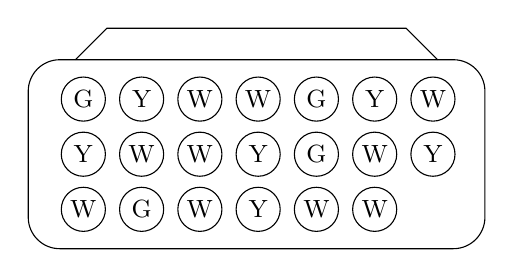
\begin{tikzpicture}[x=1mm,y=1mm]
  \draw[rounded corners=4mm] (0,0) rectangle (58,24);
  \draw (6,24) -- (10,28) -- (48,28) -- (52,24);
  \foreach \l [count=\i from 0] in {G,Y,W,W,G,Y,W,Y,W,W,Y,G,W,Y,W,G,W,Y,W,W}{
    \pgfmathtruncatemacro{\r}{\i/7}
    \pgfmathtruncatemacro{\c}{mod(\i,7)}
    \draw (7+\c*7.4,19-\r*7) circle (2.8);
    \node[font=\small] at (7+\c*7.4,19-\r*7) {\l};}
\end{tikzpicture}
\end{ealglossed}

\begin{ealglossed}
\q The \ealgloss{probability}{prawdopodobieństwo} that a train is late is 0.12. What is the \ealgloss{probability}{prawdopodobieństwo} that it is not late?
\end{ealglossed}

\begin{ealglossed}
\q The table shows the \ealgloss{probabilities}{prawdopodobieństwa} of a spinner landing on each colour. Find the \ealgloss{probability}{prawdopodobieństwo} that it lands on yellow.\\[4pt]
{\renewcommand{\arraystretch}{2.5}%
\begin{tabular}{|l|c|c|c|c|}\hline
Colour & Red & Blue & Green & Yellow\\\hline
\ealgloss{Probability}{prawdopodobieństwo} & 0.3 & 0.25 & 0.15 & \\\hline
\end{tabular}}
\end{ealglossed}

% ----------------------------------------------------------------
\begin{ealglossed}
\topic{Listing \ealgloss{outcomes}{wyników} systematically}
\end{ealglossed}

\q A caf\'e sells three starters: soup (S), melon (M) and prawns (P). It sells two mains: fish (F) and curry (C). List all the possible meals of one starter and one main.

\begin{ealglossed}
\q Spinner A is numbered 1, 2, 3, 4. Spinner B is numbered 1, 2, 3. Both spinners are spun, and the two scores are multiplied.\\
(a) Copy and complete the \ealgloss{sample space diagram}{diagram przestrzeni prób}.\\
(b) Find the \ealgloss{probability}{prawdopodobieństwo} that the answer is \ealgloss{even}{parzysty}.\\[4pt]
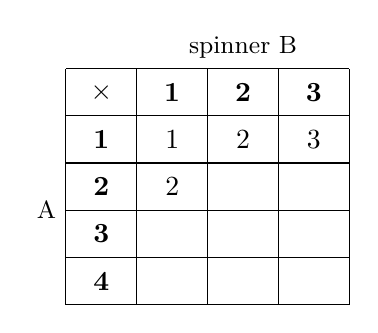
\begin{tikzpicture}[x=9mm,y=6mm]
  \draw[step={(1,1)}] (0,-4) grid (4,1);
  \node at (0.5,0.5) {$\times$};
  \foreach \b in {1,2,3}{\node at (\b+0.5,0.5) {\textbf{\b}};}
  \foreach \a in {1,...,4}{\node at (0.5,-\a+0.5) {\textbf{\a}};}
  \foreach \b in {1,2,3}{\node at (\b+0.5,-0.5) {\b};}
  \node at (1.5,-1.5) {2};
  \node[above] at (2.5,1) {\small spinner B};
  \node[left] at (0,-2) {\small A};
\end{tikzpicture}
\end{ealglossed}

% ----------------------------------------------------------------
\topic{Expected results}

\begin{ealglossed}
\q A \ealgloss{fair}{uczciwa} coin is flipped 300 times. How many heads would you expect?
\end{ealglossed}

\begin{ealglossed}
\q The \ealgloss{probability}{prawdopodobieństwo} that a bus is late is 0.08. On how many of 250 journeys would you expect the bus to be late?
\end{ealglossed}

% ----------------------------------------------------------------
\begin{ealglossed}
\topic{\ealgloss{Experimental probability}{prawdopodobieństwo doświadczalne}}
\end{ealglossed}

\begin{ealglossed}
\q A dice is rolled 200 times. The table shows the results.\\[4pt]
{\renewcommand{\arraystretch}{2.5}%
\begin{tabular}{|l|c|c|c|c|c|c|}\hline
Score & 1 & 2 & 3 & 4 & 5 & 6\\\hline
\ealgloss{Frequency}{częstość} & 31 & 35 & 30 & 36 & 33 & 35\\\hline
\end{tabular}}\\[4pt]
(a) Find the \ealgloss{relative frequency}{częstość względną} of rolling a 4.\\
(b) Do the results suggest that the dice is \ealgloss{fair}{uczciwa}? Explain your answer.
\end{ealglossed}

\begin{ealglossed}
\q Jo flips a coin 20 times and gets 14 heads. Kai flips the same coin 500 times and gets 260 heads. Whose results give the better estimate of the \ealgloss{probability}{prawdopodobieństwa} of heads? Write down this estimate.
\end{ealglossed}

% ----------------------------------------------------------------
\begin{ealglossed}
\topic{\ealgloss{Frequency trees}{drzewka częstości}}
\end{ealglossed}

\begin{ealglossed}
\q 120 people visited a museum. 70 of them were adults. 45 of the adults bought a guidebook. 20 of the children bought a guidebook.\\
(a) Copy and complete the \ealgloss{frequency tree}{drzewko częstości}.\\
(b) A visitor is chosen at \ealgloss{random}{losowo}. Find the \ealgloss{probability}{prawdopodobieństwo} that they bought a guidebook.\\[4pt]
{\renewcommand{\leafa}{Book}\renewcommand{\leafb}{No book}%
\freqtree{120}{Adults}{}{Children}{}{}{}{}{}}
\end{ealglossed}

\end{multicols}

\newpage

\begin{multicols}{2}

% ----------------------------------------------------------------
\begin{ealglossed}
\topic{\ealgloss{Venn diagrams}{diagramy Venna}}
\end{ealglossed}

\begin{ealglossed}
\q There are 50 pupils in a year group. 28 study French (F), 19 study Spanish (S), and 8 study both.\\
(a) Copy and complete the \ealgloss{Venn diagram}{diagram Venna}.\\
(b) A pupil is chosen at \ealgloss{random}{losowo}. Find the \ealgloss{probability}{prawdopodobieństwo} that they study neither language.\\[4pt]
\venn{F}{S}{}{}{}{}
\end{ealglossed}

\begin{ealglossed}
\q The \ealgloss{Venn diagram}{diagram Venna} shows the numbers from 1 to 15. A is the \ealgloss{even}{parzyste} numbers and B is the \ealgloss{square numbers}{liczby kwadratowe}. One of the numbers is chosen at \ealgloss{random}{losowo}. Find\\
(a) P($A\cap B$), the \ealgloss{probability}{prawdopodobieństwo} that it is in A and B\\
(b) P($A\cup B$), the \ealgloss{probability}{prawdopodobieństwo} that it is in A or B or both\\
(c) P($A'$), the \ealgloss{probability}{prawdopodobieństwo} that it is not in A.\\[4pt]
\venn{A}{B}{\hspace*{2mm}2\enspace 6\\[1pt]\hspace*{2mm}8\enspace 10\\[1pt]\hspace*{2mm}12\enspace 14}{4}{1\\[2pt]9}%
  {\node at (4,17) {3}; \node at (62,17) {5}; \node at (4,4) {7}; \node at (62,4) {11};
   \node at (33,31.3) {13}; \node at (33,2.7) {15};}
\end{ealglossed}

% ----------------------------------------------------------------
\begin{ealglossed}
\topic{\ealgloss{Conditional probability}{prawdopodobieństwo warunkowe} with \ealgloss{Venn diagrams}{diagramy Venna}}
\end{ealglossed}

\begin{ealglossed}
\q The \ealgloss{Venn diagram}{diagram Venna} shows 60 people, and whether they own a cat (C) or a dog (D).\\[4pt]
\venn{C}{D}{14}{10}{21}{\node at (60,4) {15};}\\[2pt]
(a) Find the \ealgloss{probability}{prawdopodobieństwo} that a person chosen at \ealgloss{random}{losowo} owns a dog.\\
(b) \ealgloss{Given}{pod warunkiem, że} that a person owns a dog, find the \ealgloss{probability}{prawdopodobieństwo} that they also own a cat.
\end{ealglossed}

\begin{ealglossed}
\q Use your \ealgloss{Venn diagram}{diagramu Venna} from question 11. \ealgloss{Given}{pod warunkiem, że} that a pupil studies French, find the \ealgloss{probability}{prawdopodobieństwo} that they also study Spanish.
\end{ealglossed}

% ----------------------------------------------------------------
\topic{Problem solving}

\begin{ealglossed}
\q A bag holds red and blue counters in the \ealgloss{ratio}{stosunku} $3:5$. Two more red counters are put in the bag. Now the \ealgloss{probability}{prawdopodobieństwo} of taking a red counter is $\frac12$. How many counters were in the bag at the start?
\end{ealglossed}

\begin{ealglossed}
\q A spinner has 5 equal sections, each coloured red, blue or green. The \ealgloss{probability}{prawdopodobieństwo} of red is 0.4, and the \ealgloss{probability}{prawdopodobieństwo} of blue is twice the \ealgloss{probability}{prawdopodobieństwo} of green. Draw the spinner.
\end{ealglossed}

\begin{ealglossed}
\q Sam rolls a dice 6 times and never gets a 6. He says, ``The dice must be \ealgloss{biased}{obciążona}.'' Is Sam right? Explain your answer.
\end{ealglossed}

\end{multicols}

\end{document}